Generar un lazo de control que tenga como entrada la velocidad de referencia, y que contemple las perturbaciones externas del sistema en el cálculo de la velocidad de salida que se utilizará como lazo de realimentación. 
Adaptar la acción de control que ingresa al variador de velocidad (adquirido por el Laboratorio de Fluidos) para alimentar al motor y dejar en desuso el banco de resistencias que se utiliza.
Además, realizar una interfaz gráfica para un mejor manejo y control del sistema.

\begin{figure}[htb]
	\centering
	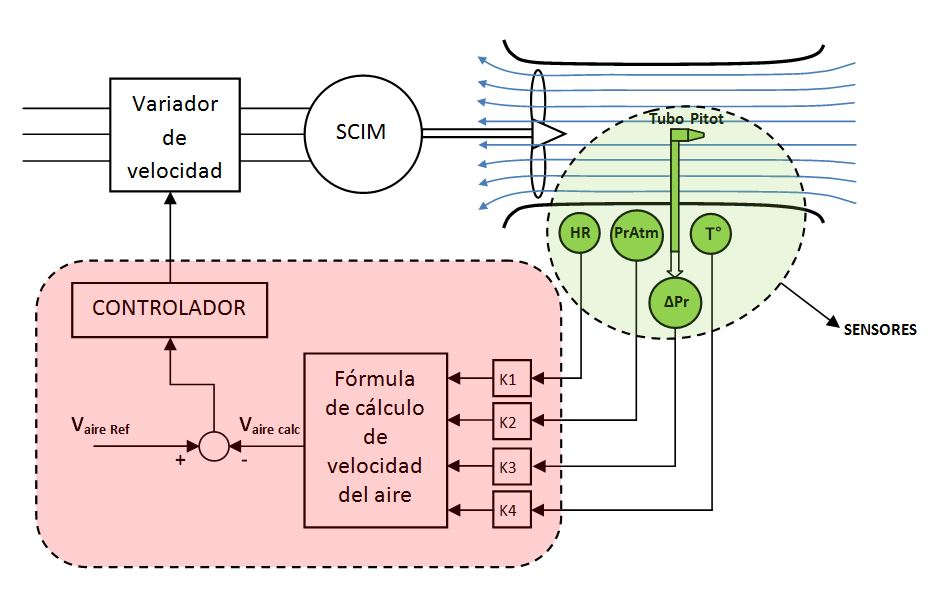
\includegraphics[scale=0.35]{diagr.jpg}
	\caption{Diagrama}
	\label{fig:diagr}
	\end{figure}